%نام و نام خانوادگی:
%شماره دانشجویی: 
\مسئله{}
در ارتباط با رابط کاربری و تجربه‌ی کاربری:
\begin{enumerate}[a)]
	\item 
تفاوت رابط کاربری \footnote{\lr{User Interface}} و تجربه‌ی کاربری \footnote{\lr{User Experience}} چیست؟
	\item 
پنج مورد از نقاط قوت و پنج مورد از نقاط ضعف در طراحی رابط و تجربه‌ی کاربری سامانه‌ی آموزش دانشگاه را بیان کنید.‌
\end{enumerate}

\پاسخ{
\begin{enumerate}[a)]
	\item 
تفاوت اصلی این دو در تمرکز اصلی‌شان و نحوه‌ی برقراری ارتباط کاربر با آن‌ها است که درادامه به تفصیل درموردشان صحبت می‌کنیم.
	
رابط کاربری درمورد طراحی، معماری اطلاعات و بخش‌های بصری یک محصول مانند صفحات، دکمه‌ها، رنگ‌‌ها و منوها است که کاربر به هنگام استفاده از محصول مستقیما با آن‌ها تعامل برقرار می‌کند. تمرکز رابط کاربری روی بهینه‌سازی این ارتباط و کیفیت محصول است و تنها درمورد محصولات دیجیتال به کار می‌رود. می‌توان گفت که رابط کاربری بخشی از تجربه‌ی کاربری را تشکیل می‌دهد (البته نه به صورت کامل).

تجربه‌ی کاربری مفهومی کلی و انتزاعی است که درمورد تجربه‌‌ی کاربر از قبل تا بعد از خرید و کار با محصول به‌کار می‌رود. تجربه‌ی کاربری روی این تمرکز می‌کند که محصول قابل استفاده (Functional) ، در دسترس و کاربرپسند \footnote{User-friendly} باشد. این مفهوم را می‌توان هم درمورد محصولات دیجیتال و هم غیردیجیتال استفاده کرد. برای فراهم کردن تجربه‌ی کاربری خوب، باید نیازها، مشکلات‌ و اهداف مشتریان را درک کرد و محصولی تولید کرد که این نیازها را برآورده کند و کار کردن با آن لذت‌بخش و آسان باشد. تجربه‌ی کاربری علاوه بر رابط کاربری و بخش‌هایی از محصول که کاربر با آن‌ها در ارتباط است، نحوه‌ی ارتباط این بخش‌ها بایکدیگر و انتقال کاربر بین آن‌ها را هم دربر می‌گیرد.

برای شفاف‌تر شدن تفاوت بین این دو از یک مثال استفاده می‌کنیم. فرض کنید که در یک کافه قهوه سفارش می‌دهید. در این صورت قاشق، شکر و مواد دیگری که همراه با قهوه به شما تحویل داده‌می‌شوند مربوط به تجربه‌ی کاربری هستند و هدف‌شان بهتر کردن تجربه‌ی شما و برآورده کردن تمامی نیازهایتان است. درکنار آن رنگ فنجان، قاشق و طرح میزها مربوط به رابط کاربری هستند و به ایجاد لذت بصری کمک می‌پردازند. 
\begin{figure}[h]
	\centering
	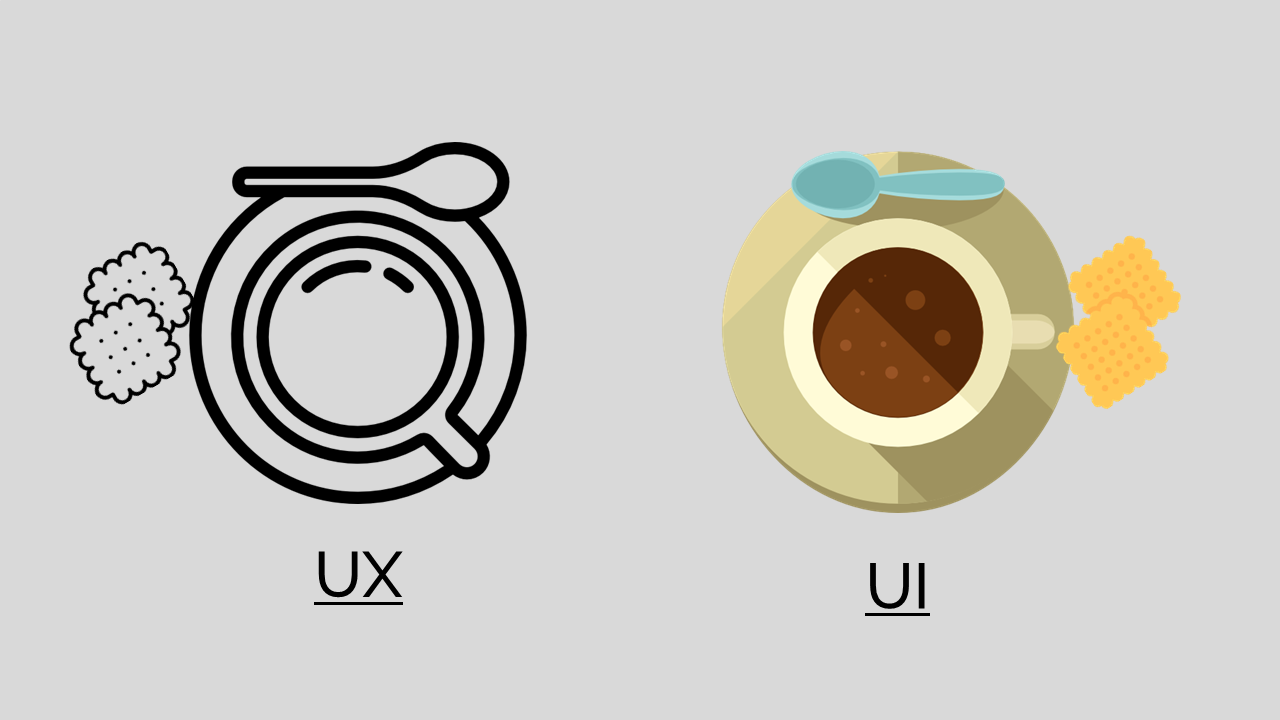
\includegraphics[scale=0.32]{figs/6_1}
	\caption{تفاوت رابط کاربری و تجربه‌ کاربری در مثال کافه}
\end{figure}
\newpage
تفاوت‌های این دو مفهوم به خلاصه در جدول زیر نیز آورده‌شده‌اند:
\begin{center}
    \begin{tabular}{ | r | p{8cm} |}
    \hline
   رابط کاربری & تجربه کاربری \\ \hline
   دید جزئی به محصول & دید کلی به محصول \\ \hline
  جنبه‌های ملموس و قابل دیدن طراحی & جنبه‌های انتزاعی طراحی \\ \hline
    محصول چگونه به‌نظر می‌رسد & استفاده از محصول چه حسی در کاربر ایجاد می‌کند \\ \hline
    بعد بصری تجربه‌ی کار با محصول & تمامی ابعاد تجربه‌ی کار با محصول \\ \hline
    تمرکز روی طراحی سطوح تعامل کاربر  & تمرکز روی تشخیص نیازمندی‌های کاربر و ارائه‌ی راه‌حل‌های ساختاری \\ \hline
  تمرکز روی طراحی محصول نهایی & تمرکز بر مراحل ایده‌پردازی، توسعه و ارائه محصول و تجزیه و تحلیل \\ \hline
    محصولات دیجیتال &  محصولات دیجیتال و غیردیجیتال \\ \hline
    
    \end{tabular}
\end{center}

درنهایت باید تاکید کرد که رابط کاربری و تجربه‌ی کاربری مکمل یکدیگر هستند و هردو برای تولید یک محصول رضایت‌بخش ضروری‌اند و نمی‌توان یکی را به دیگری ارجحیت داد.
	\item 

\end{enumerate}


\subsection*{مراجع}

\begin{latin}
	\begingroup
	\renewcommand{\section}[2]{}%
	
\begin{thebibliography}{9}
%   Check this for adding items: https://www.student.unsw.edu.au/how-do-i-cite-electronic-sources
	\bibitem{Coursera}
	\textit{UI vs. UX Design: What’s the Difference?},
	Accessed on 1/10/2023,
	\url{https://www.coursera.org/articles/ui-vs-ux-design}
	
	\bibitem{Master's in Data Science}
	\textit{What is the difference between UX and UI?},
	Accessed on 1/10/2023,
	\url{https://www.mastersindatascience.org/learning/difference-between-ui-and-ux/}
	
	\bibitem{UX Design Institute}
	\textit{UX vs. UI design: What’s the difference?},
	Accessed on 1/10/2023,
	\url{https://www.uxdesigninstitute.com/blog/ux-vs-ui-design/}
	
	\bibitem{RTL-THEME}
	\textit{UX and UI Difference},
	Accessed on 1/10/2023,
	\url{https://www.rtl-theme.com/blog/ux-ui-difference/}
\end{thebibliography}
\endgroup
\end{latin}

}
